HTBAC serves as a software tool to enable ensemble-based free energy
protocols to run adaptively and at scale.

% \mtnote{protocols?}\jdnote{addressed}.

% HTBAC is based on a co-design which integrates users i.e. domain experts
% and developers to elicit requirements.

% \mtnote{I am not sure I understand what this means. Domain experts and
% developers both elicit requirements? What about the rest of the development
% process? The sentence's grammar also needs attention}.

% The co-design process is iterative. For example, certain features become
% available during the software lifetime which in turn can be used by domain
% experts to build new algorithms that require such features.

% ---------------------------------------------------------------------------
\subsection{Requirements}

HTBAC has three primary requirements: (1) enable the scalable execution of
concurrent free energy protocols; (2) abstract the complexity of building
protocols from execution and resource management; and, (3) provide adaptivity
by modifying the task-graph at runtime to enable more efficient protocol
runs.

Computational drug campaigns increasingly depend on scalable ensemble-based
protocols. This pose at least two major computational challenges: First,
ensemble-based protocols require execution coordination and resource
management among ensemble members, within protocols as well as across
protocols. Second, the setup of execution environments and data management
has to preserve efficient resource utilization. These challenges need to be
addressed by HTBAC as well as the underlying ensemble management and runtime
system.

Adaptivity is another feature required by modern computational drug
campaigns. Adaptive protocols allow to change the control logic of the
ensemble execution, based on intermediate results of the ongoing computation.
Thus, HTBAC will have to support the redistribution of resources, according
to the logic provided by the adaptive algorithms. In this way, HTBAC will
maximize computational efficiency.

Finally, usability plays an important role in the development of HTBAC. HTBAC
has to provide a flexible interface which enables users to easily scale the
number of drug candidates and quickly prototype existing and novel free
energy protocols.

% \mtnote{``from'' instead of ``,''? See also comment in the following
% paragraph}

% (i.e., modifying the task-graph at runtime, based on previous tasks), to
% enable efficient protocols and effective resource sharing across and within
% protocols. without explicit resource management requirements.

% \mtnote{Grammar: the sentence as it is is incorrect. For example, note the
% use of `this' after a `,', the repetition of requirements/require.}.
% \jdnote{re-phrased}

% \jdnote{reworded this paragraph and hesitant to say workload management
% system.}\mtnote{avoiding WMS is fine by me. Unfortunately, the paragraph
% still does not read well. I would have another go at it but please let me
% know whether you want me to suggest an alternative version.}
% \jdnote{I changed the first sentence but I'm not sure what you doesn't read
% well}

% \mtnote{which one?}\jdnote{keeping it general to campaigns}

% and minimal overhead workload management system and the runtime system
% (RTS) that support HTBAC.

% \mtnote{I am not sure I understand this sentence: grammar
% (``Based\ldots,this''?; and from the previous paragraph, we say that HTBAC
% abstracts the complexities of execution and resource management but here we
% focus on WMS and RTS? Are WMS and RTS components of HTBAC?}

% The RTS has to provide sustainable submission and tracking of heterogeneous
% protocols i.e.\mtnote{note: ``i.e.'' cannot be place in the middle of a
% sentence without supporting punctuation} protocols that differ in
% computational requirements, as well as setup of execution environments and
% data management while preserving efficient resource utilization and minimal
% overhead.\mtnote{Why this is relevant for HTBAC?}

% \mtnote{which algorithm? This paragraph seems disconnected
% from the previous one.} \jdnote{changed}

% may decide to invest additional compute resources in simulations that can
% yield lower error averages, while reducing resources for simulations that
% have already met an error threshold. HTBAC thereby requires % an adaptive
% execution strategy \mtnote{system}

% \jdnote{changed from adaptive RTS to adaptive execution strategy}
% \mtnote{`execution strategy' is also undefined here. I simplified, please
% revert if incorrect.}\jdnote{kept the previous writing of this idea
% commented} 

% that enables adaptive algorithms to maximize computational efficiency.

% \mtnote{Seeing that we are speaking about requirements, does it make sense
% here to mention a RTS? RTS are an implementation detail: for example, we
% could design HTBAC as an end-to-end solution for a specific machine and
% still match the set of requirements we have reported in this subsection.
% Note also that we introduce RTS above but use ``runtime system'' again
% here.}\jdnote{I've removed all mention of workload management system and
% RTS and kept generality}

% Included in usability is the abstraction of adaptive features, to
% enable users to design protocols that utilize adaptive functionality to
% leverage intermediate results.
% \mtnote{The second sentence of the paragraph might be a repetition of what
% already wrote in the previous paragraph.}
% \jdnote{I can see that, but wanted to explicitly highlight the adaptive
% features as part of usability.}

% ---------------------------------------------------------------------------
\subsection{Design}

HTBAC exposes the following user-facing constructs to enable users to specify
free energy protocols in terms of ensemble applications:

\begin{itemize}
  \item \textbf{Protocol:} A generic abstraction of a free energy protocol
  such as ESMACS or TIES.
  \item \textbf{Simulation:} Simulation parameters that supply additional
  information for each protocol instance.
  \item \textbf{Runner:} A generic abstraction to describe resources needed
  by the application.
\end{itemize}

The \textbf{Protocol} construct enables multiple instantiations of protocol
types, while the \textbf{Simulation} construct specifies simulation
parameters that shape each protocol. The \textbf{Runner} construct provides
the functionality to specify the resource requirements and the amount of time
these resources should be available to execute the application. Thus, in
HTBAC an application consists of protocols, simulation conditions, and
resource requirements.

\mtnote{The following is about architecture and execution model: ``HTBAC rests between the domain scientist and the cyber-infrastructure,
abstracting the complexity of encoding end-to-end protocols, resource
acquisition and execution management. The Runner initializes HTBAC and holds
the global state of the application, submits protocols and communicates with
the ensemble management system that handles the dependencies of the
protocols, and acquires resources via a runtime system.''}

In HTBAC, an application can have one or more protocol instance(s). Each
protocol models a unique protein ligand physical system. Each protocol
follows a sequence of simulation and analysis steps and assigns ensemble
members to execute independent simulations or analysis. An ensemble member
that executes an independent simulation within a simulation step is referred
to as a \textbf{replica}. Each replica simulation is assigned a different
initial velocity, which enables simulations to begin in different parts of
the ligand's phase space.

An individual simulation or analysis is a computational \textbf{task}, with
well-defined input, output, termination criteria and dedicated
resources~\cite{power-of-many17}. Aggregates of tasks with dependencies that
determine the order of their execution describe \textbf{workflows}. A
workflow is comprised of $N_P$ instances of the P$^{th}$ protocol. In this
way, workflows in HTBAC encode the description of the scientific problem in
terms of computational tasks.

% \subsubsection{Application Model}

% \mtnote{what is an ``application of HTBAC''? `In' (instead of `of')
% HTBAC?}\jdnote{addressed}

% \mtnote{``resource abstraction of the application''? Resources for the
% application?}\jdnote{addressed}

% \mtnote{what is the relation among protocol, simulation and application?}.
% \jdnote{changed sentence.}

% \mtnote{we used `construct' before, as a synonym of abstraction}\mtnote{we
% used `construct' before, as a synonym of abstraction}\jdnote{I've removed
% any reference to object-orientation and kept everything to construct in
% design but in implementation it changes to components}

% \subsubsection{Architecture}

% \mtnote{The runner here seems to be a component: it initializes, holds,
% submits, etc.}
% \jdnote{Given that this section is Design, I referred to Runner as a
% construct. But maybe this sentence belongs more in Architecture?}

% \mtnote{The following is part of design. I would move it up and collate.
% See my comment in the previous subsection asking for the relation between
% protocol and application. I did not understand that relation until I read
% the following.} \jdnote{moved to Design}

% \mtnote{see the previous comment about using `i.e.'}\jdnote{removed i.e.}

% \jdnote{does this confuse the term application with workflow?}\mtnote{It
% doesn't but it is on us to define the relation between an application and a
% workflow.}\jdnote{Looked at EnTK to understand the relations}

% Workload: A set of tasks, possibly related by a set of arbitrarily complex 
% relations. For example, relations may involve tasks, data, or runtime 
% communication requirements 

% \mtnote{End of part to move up to design.}


% ---------------------------------------------------------------------------
\subsubsection{Architecture}

\jdnote{started an Architecture section but need input on how to describe 
the API, and application management layer, given that all the components are 
mixed between both. The runner is the main component of the application 
management layer because it is the driver that collects the protocols and 
submits them to EnTK. Would it make sense to show 3 layers then? API, 
application management and protocol generation?} 

HTBAC abstracts the resource management and execution management from the user. 
Figure~\ref{fig:components} shows the components and subcomponents of the 
HTBAC. All three components enable the user to codify an application 
description of HTBAC. The runner serves as the application management system,
by initializing the state of the application and communicating with the 
ensemble management system. 

Figure~\ref{} shows a visual block diagram representation \mtnote{`visual
block diagram representation' seems unclear to me. Should we just have an
architecture diagram here?} of HTBAC and the underlying building
blocks.\jdnote{adding architecture diagram -- in draft
currently}\mtnote{Note: architecture diagrams are static. They can be
`augmented' with numbers (and often arrows) to support the description of an
execution model. Please review a couple of papers the group wrote with this
type of diagram.} \jdnote{working on architecture with execution model 
diagram. For now I'm referencing component and subcomponent diagram}

\begin{figure}
  \centering
  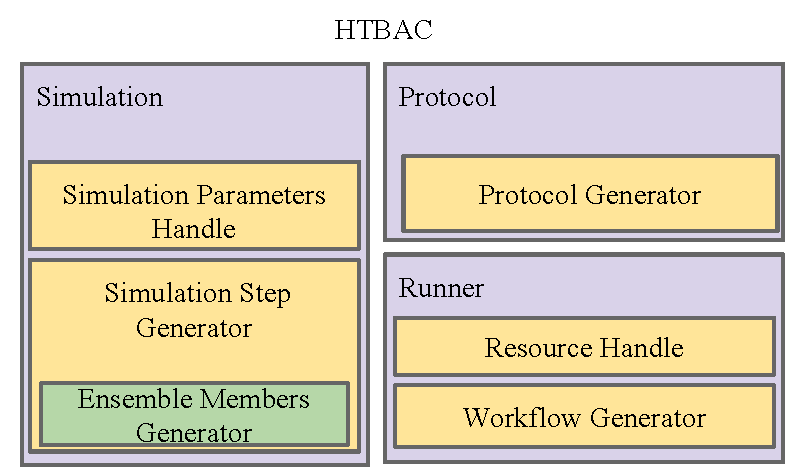
\includegraphics[width=\columnwidth]{figures/Component_Subcomponent_Diagram.pdf}
  \caption{Components and subcomponents of HTBAC. The protocol, simulation and 
  runner are the main components. The protocol and simulation components 
  describe the protocols and their simulation conditions. The runner component 
  serves as the application manager by interfacing with the ensemble management 
  system.}
\label{fig:components}
\end{figure}

% ---------------------------------------------------------------------------
% Protocols differ only by their individual analysis step which typically
% follows production simulation and by the computational requirements,

% see figure X for a visual representation of the ESMACS and TIES workflows
% \mtnote{grammar. I am not able to follow the sentence}.

% Moreover the \textbf{Simulation} class provides the granularity to specify
% individual parameters per replica, including the number of cores per
% replica, MD execution kernel and the length of each simulation
% step.\mtnote{This might be seen more as a description of the implementation
% of HTBAC instead of its design}\jdnote{moved this to TIES description of
% implementation}

% Note that some protocols require additional information. For example, the
% TIES protocol contains additional sampling parameters or $\lambda$ windows.
% Moreover, the \textbf{Simulation} class exposes a method which enables the
% user to codify new algorithms, or modify an existing protocol such as
% specifying additional equilibration or analysis steps.\jdnote{move to
% implementation}

% Once the protocols and simulation parameters are defined, they are passed
% to the \textbf{Runner} class where the user defines the resource
% requirements including cyber-infrastructure and duration of the application
% as well as additional flags for adaptive execution which are passed down by
% the \textbf{Runner} to the workload management and runtime
% systems.\mtnote{This seems to be mixing implementation, execution flow and
% architecture?}
% ---------------------------------------------------------------------------

\mtnote{General note. It may be useful to recall the difference between
software architecture and software design. Software architecture is about the
structure of the software system, with a particular focus on modularity and
how it is rendered by components and interfaces (e.g., communication and
coordination protocols). Software design is about defining the
functionalities of each module, \textbf{showing} (i.e., arguing for) how
these functionalities address the requirements. In this context, the notion
of `class' and `method' are often regarded as implementation details, even if
object-oriented design is indeed one of the many ways to approach software
design. More in general, both architecture and design can be expressed with a
varying degree of formality and many different patterns and languages have
been and are still being developed. In this paper, we just use plain English,
informal diagrams, and a very high level overview. This approach should not
be confused with lack of precision or of scientific rigor: the goal of this
paper is to show how HTBAC architecture and design support better science in
a very specific domain, not to argue for their rigorous nature.}
\jdnote{I've modified the design to be more consistent in showing
functionality of constructs and separated architecture design from
application model}

% Each replica follows the same sequence of simulation steps including
% minimization, equilibration and production simulation.\mtnote{see the
% previous comment about using `i.e.'}\jdnote{addressed}

% For TIES, where each protocol  corresponds to a single physical system. The
% TIES protocol object enables the user to select a physical system, number
% of replicas, core allocation per replica, and $\lambda$ windows to sample.
% Figure~\ref{fig:pst} provides the visual implementation of the TIES
% protocols into the PST model.

% ---------------------------------------------------------------------------
\subsection{Implementation}

% The \textbf{Protocol} construct is the main abstraction of HTBAC. 

HTBAC is a domain specific library implemented in Python. All components of
HTBAC are implemented as objects. Communication in HTBAC occurs by function
calls, either by value or reference. HTBAC uses the RADICAL-Cybertools (RCTs) as 
building blocks~\cite{review_bb_2016} to support HTBAC's workflow execution 
across diverse computing platforms~\cite{turilli2017comprehensive}. HTBAC rests 
on two primary RCT libraries: Ensemble Toolkit (EnTK) and RADICAL-Pilot (RP).

EnTK provides an application model that simplifies both the encoding and
execution of scalable and adaptive free energy protocols that differ in
computational requirements. EnTK exposes 3 user-facing constructs:
\textbf{Task}, \textbf{Stage} and \textbf{Pipeline}~\cite{power-of-many17}.
Tasks contain information regarding an executable, its software environment
and its data dependencies. Stages are sets of tasks without mutual
dependencies and that can be executed concurrently. Pipeline are lists of
stages where any stage $i$ can only be executed after that stage $i - 1$ has
been executed. Each pipeline can execute independently.

EnTK serves HTBAC as the ensemble management system that provides specific
interfaces and execution models for ensemble-based
applications~\cite{power-of-many17}. HTBAC uses the programming model of EnTK
to construct workflows. In HTBAC, a protocol instance is encoded as a single
pipeline, which contains stages of simulation and analysis steps. Replicas or
analysis tasks are bundled as tasks within a stage. We show the
implementation of two types of protocol types, ESMACS and TIES.\mtnote{The
previous paragraph seemed to me a mix of two paragraphs. I separated them,
feel free to revert if I did not get it right.}\jdnote{noted}

EnTK uses the runtime system of RADICAL-Pilot to execute ensemble applications 
via pilots. Pilots provide a multi-stage execution mechanism: Resources are 
acquired via a placeholder job and subsequently used to execute the 
application’s tasks~\ref{power-of-many17}. The pilot abstraction supports the 
requirements of task-level parallelism and high-throughput as needed by the use 
cases. A pilot abstraction uses a placeholder job without any tasks assigned to 
it. It acquires resources from the CI by submitting a (container) job and waits 
in the queue until the CI's scheduler bootstraps the job to the compute nodes. 
Once the pilot is scheduled, it can pull computational tasks for execution. 
This enables the tasks to be executed directly on the resources, without being 
queued via the local resource management system or without circumventing the 
queue policies of HPC resources~\ref{dakka2017}. 


\mtnote{What about RP? We write that the two relevant RCT libs are EnTK and
RP but we then introduce only EnTK explaining how HTBAC uses it.}
\jdnote{Added background, but in general how much of RP's details should go in?}

% ---------------------------------------------------------------------------
\subsection{ESMACS and TIES}

\jhanote{As written, this sub-section has nothing about HTBAC and would be better
placed/merged in Science Driver.  What would be useful is psuedo-code or code listing to show how ESMACS and TIES are encoded in HTBAC}

While ESMACS and TIES protocols compute binding affinity calculations for
different systems and purposes, their implementation in HTBAC have the same
underlying pattern, consisting of simulations steps, followed by one or more
analysis step(s). In this paper, we focus on the default sequence of
simulation steps which consist of minimization, initial equilibration,
secondary equilibration, and production MD simulation. Designers of free
energy protocols are not bound by this sequence and can utilize the Protocol
component of HTBAC to enable arbitrary sequences. 

Figure~\ref{fig:ties_esmacs_application} shows the implementation of the
ESMACS and TIES protocols. ESMACS contains 25 replicas per simulation step
while TIES contains a $\lambda$ sampling parameter which generates 5 replicas
per $\lambda$ window. In this paper, we implement TIES with 13 $\lambda$
windows to spawn a total of 65 replicas in each simulation step.

\begin{figure}
  \centering
  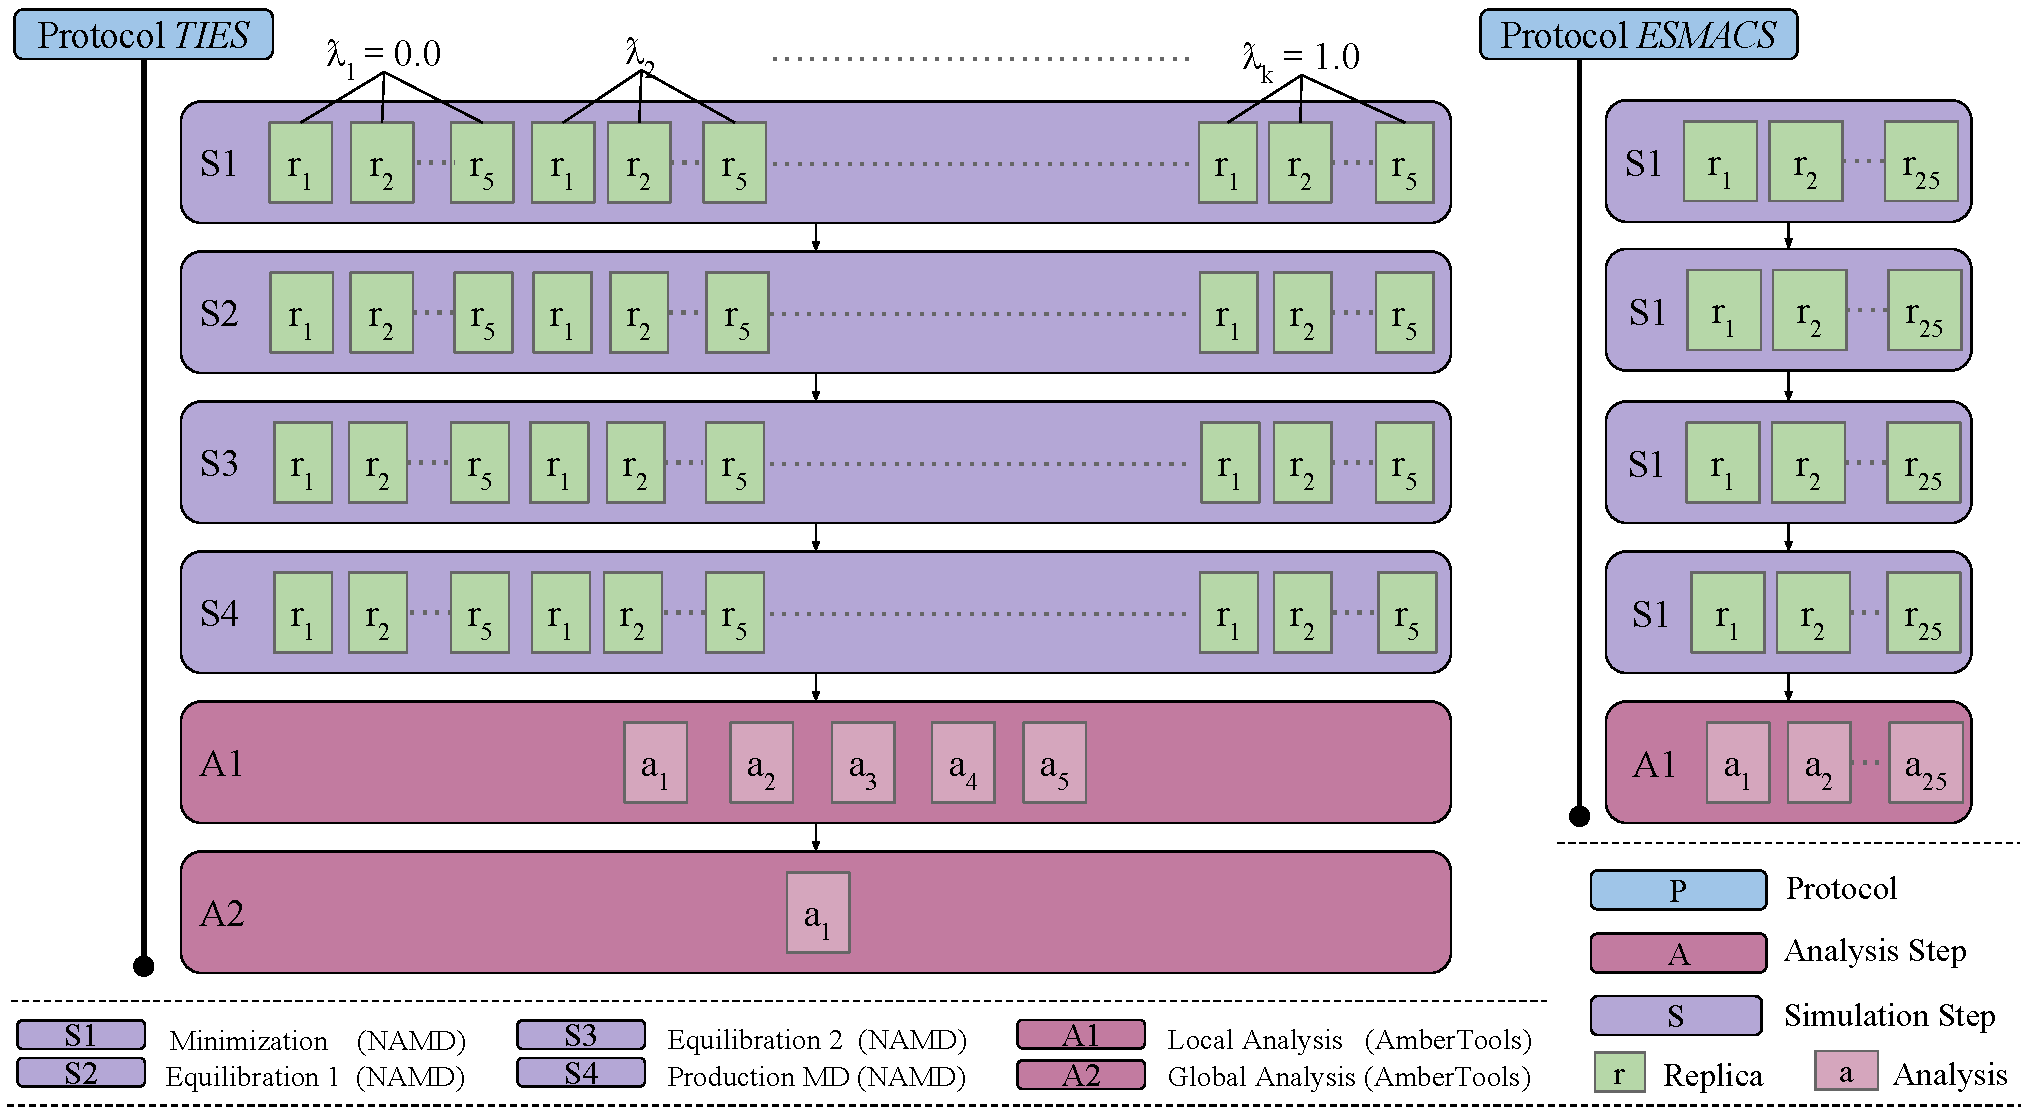
\includegraphics[width=\columnwidth]{figures/ties_esmacs_application_model.pdf}
  \caption{TIES and ESMACS protocols consist of simulations steps followed
  by analysis step(s). All replicas within a simulation step are assigned the
  following simulation timesteps, for 6 nanoseconds simulation duration:
  $S1=1000$; $S2=30,000$; $S3=800,000$; $S4=2,000,000$.}
\label{fig:ties_esmacs_application}
\end{figure}

The analysis step(s) vary according to each protocol. ESMACS contains a
single analysis step with 25 tasks that computes the MMPBSA with respect to
each replica.\jdnote{MMPBSA needs to be defined in feprotocol} TIES contains
two analysis steps. The first step is a local analysis containing 5 tasks
that aggregate the simulation results of each replica using the Hamiltonian
derivative calculation. This is followed by a global analysis stage that
contains a single task to calculate the thermodynamic integration across
replicas.

% In HTBAC, each replica is encoded as a pipeline, which contains stages of
% simulation steps. Each stage contains a single task which performs a
% simulation. Each protocol consists of an aggregate of replicas, or
% independent pipelines.

% ---------------------------------------------------------------------------
\subsection{Intra-protocol Adaptivity} 

\jhanote{Also, as written, this has nothing to do HTBAC. These are details 
about algorithms, none of which is specific to their implementation in HTBAC.
I think we need a different section that discusses how HTBAC is used to
support adaptivity in the context of TIES.}

% Protocols that have the ability to The flexibility at the protocol
% component enables the user to modify the simulation steps.

\mtnote{As agreed yesterday, I started to edit heavily the text.}

Protocol like ESMACS or TIES can be implemented via a workflow with or
without adaptivity. The nonadaptive implementation specifies all the
requirements of the protocol prior to execution. The adaptive implementation
provides instead partial requirements before execution but ``learns'' the
remaining requirements during execution.

Intra-protocol adaptivity relies on the intermediate results \textit{within}
a protocol instance to define the next set of requirements. In this paper, we
use an intra-protocol adaptive implementation of TIES because, as indicated
in section~\ref{sec:science-drivers}, the optimal positions of the $\lambda$
windows are not known \textit{a priori}. Therefore, the number of simulations
and their descriptions, which are dictated by the $\lambda$ windows
parameter, cannot be specified before execution \mtnote{`cannot be specified'
or `cannot be effectively specified'? If the former, then would that imply
that a nonadaptive implementation is not possible?}.

Figure~\ref{fig:adaptive_ties} shows our implementation of TIES as a workflow
with an iterative pipeline of two stages: a simulation step followed by an
analysis step which determines optimal placement \mtnote{is placement the
correct term here? In the previous paragraph we wrote about number of
simulations and their description, not about their placement} of further
simulations. We initialize the workflow with $y$ evenly-spaced $\lambda$
windows, which generates $y \times n$ initial replicas. After the first
simulation step, the analysis step operates on the simulation results to
determine the next placement of $\lambda$ windows and to generate a second
simulation step with new configurations. 

Each simulation step consists of multiple tasks that simulates 1 nanosecond
of \ldots \mtnote{please add here what we are simulating}. The analysis
consists of a single task that computes adaptive quadrature calculations (as
defined in section~\ref{sec:science-drivers}) to determine whether to spawn
additional $\lambda$ windows \textit{in between} existing windows. This
enables continuous execution of existing simulations and beginning of new
simulations \mtnote{I do not understand this sentence. Can we eliminate it?}.
The workflow is executed iteratively until the total simulation duration
defined by the user is reached, determining termination.

\begin{figure}
  \centering
  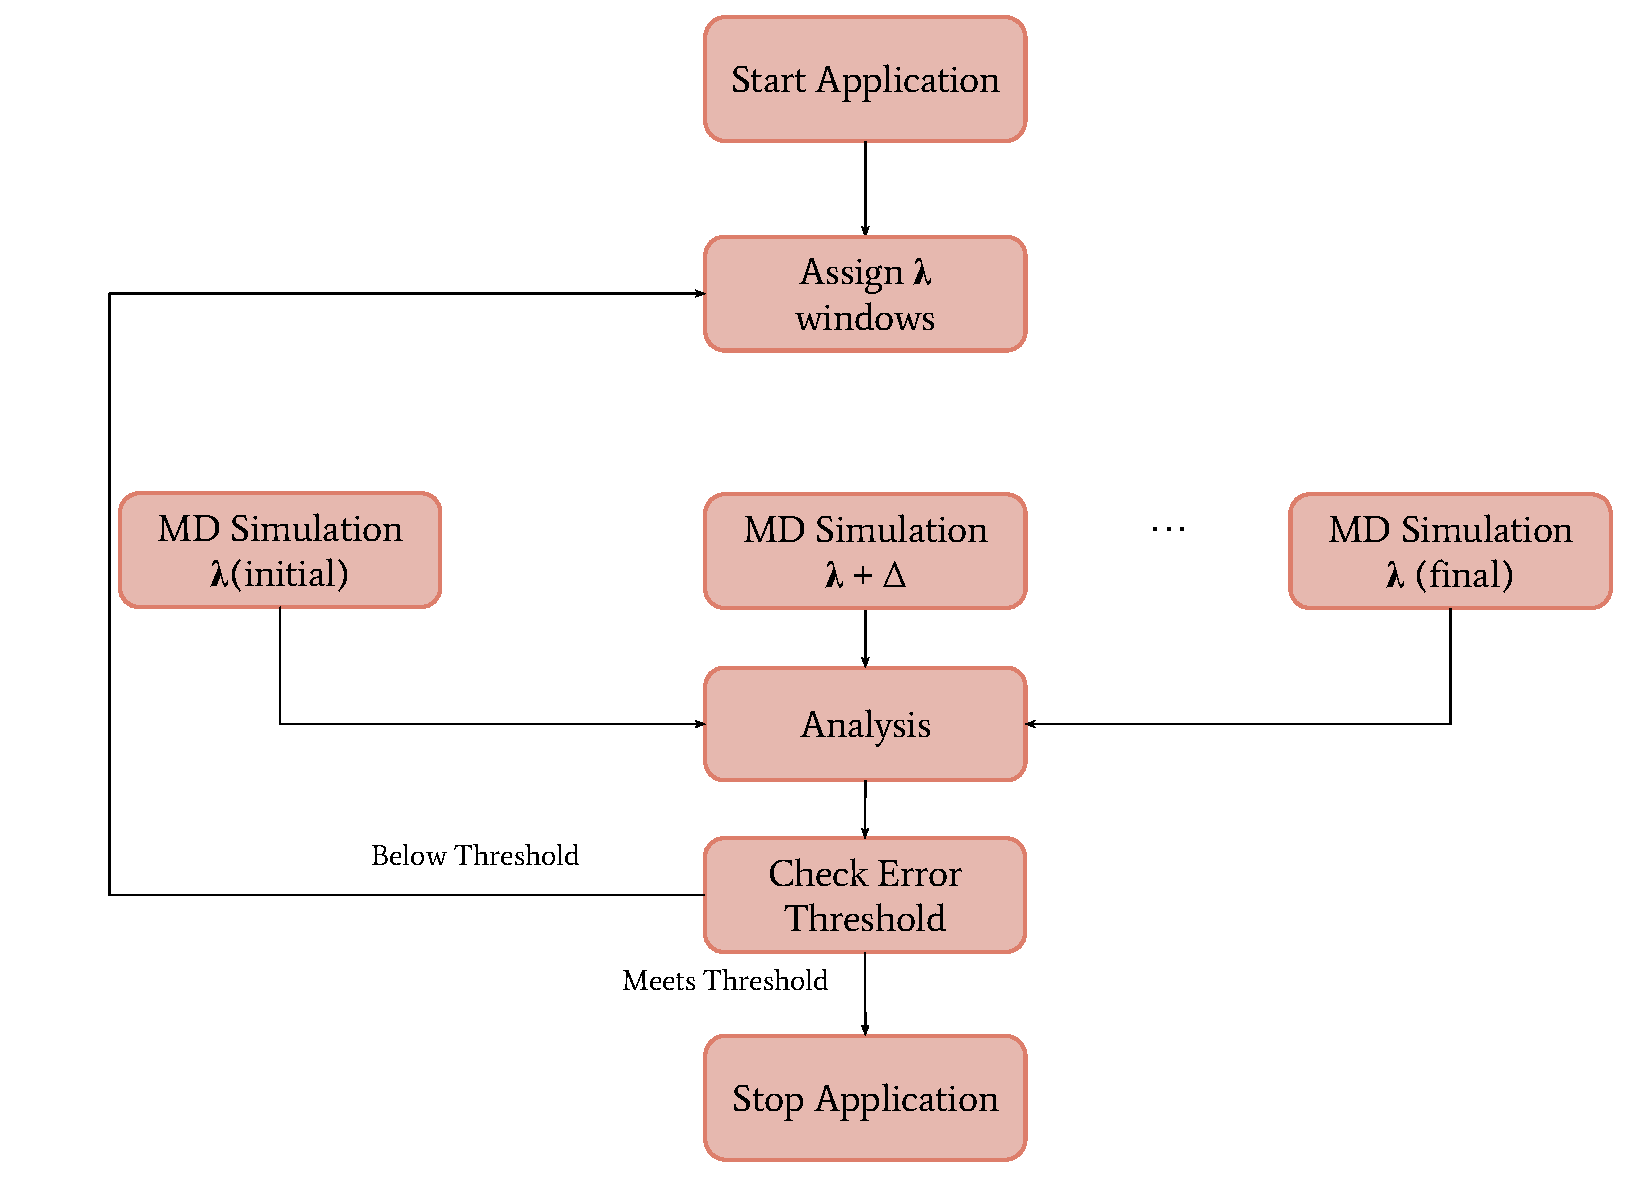
\includegraphics[width=\columnwidth]{figures/adaptive_TIES_workflow_diagram.pdf}
  \caption{Adaptive workflow of TIES with multiple concurrent and independent
  simulations. The analysis (adaptive quadratures) operates on a snapshot of
  the current simulations for each $\lambda$ window, and decides whether the
  critical threshold is reached, else current simulations continue executing
  and new simulations are spawned based on additional $\lambda$ values.}
\label{fig:adaptive_ties}
\end{figure}

% ---------------------------------------------------------------------------
\subsection{Execution Model}

Once an adaptive or nonadaptive workflow is described in HTBAC, the Runner
component tags each protocol instance with a unique ID and converts protocols
into EnTK pipelines or stages of tasks. Pipelines are submitted to EnTK's
Application Manager component which sets up multiple processes, threads and a
message queue for communication. EnTK identifies tasks which have satisfied
dependencies and can be executed concurrently. EnTK's Execution Manager
component uses its underlying runtime system (RP) to execute the tasks of the
pipelines on specific target resources.

% \mtnote{the previous paragraph does not mention workflow(s) so this
% surprises and confuses the reader. Note that this is a byproduct of
% commenting out part of the text where a connection between protocol and
% workflow was explicitly established}\jdnote{provided earlier definition of
% workflows},

The Runner component of HTBAC also describes the computational requirements
of the workflow including walltime, cores, queue, and user credentials. EnTK
uses these requirements to derive a resource request that is then converted
into a pilot description for RP. RP converts this pilot requests into a batch
script that is submitted to a suitable HPC machine. Once the pilot becomes
active, it pulls the tasks made available by EnTK in bulk, executing them on
the pilot resources~\cite{merzky2015radical}.

% ---------------------------------------------------------------------------
\subsection{Adaptive Execution Model}

Support for intra-protocol adaptive workflows requires an adaptive execution 
strategy. We leverage the adaptive capabilities provided by 
EnTK~\cite{adaptivebiomolecular} to raise the level of adaptive features 
abstraction in HTBAC. The intra-protocol adaptivity schema requires the 
redistribution of resources to account for additional simulations generated 
during runtime. 

% As demonstrated by the requirements of the TIES intra-protocol 
% adaptivity schema, the runtime system that provisions resources to support 
% execution of concurrent simulations will need to redistribute resources in order 
% to support concurrent execution of both existing and new simulations. 

Using the protocol, runner, simulation components, users express the initial 
protocol configuration and resource requirements. The user also provides the 
analysis script that is required to generate simulations configurations during 
runtime decisions. 

% The workflow method exposed by
% the protocol component enables granularity in creating multiple ``shorter" 
% protocols. 

The runner maintains the state of the submitted protocol by tagging each 
protocol instance with a unique ID. This enables the runner to keep track of
protocol instances that require additional simulations. 
% The protocol component 
% contains a post-execution property that invokes the application once the protocol 
% terminates. In HTBAC, the 

Once simulations have executed, a post-execution property of the protocol object
performs a write operation of the simulation results. After the initial protocol 
executes, the control logic returns back to the main script where the user has 
already pre-specified an analysis script that computes the next placement of 
simulations based on the output generated by the protocol. The choice of this 
strategy is to account for various functionalities that are specific to the 
requirements of the user. The protocol component contains a parameter that 
accepts new simulation conditions and builds a new workflow that extends the 
current protocol by incorporating new simulations.

As the number of simulations grows during runtime, the ratio of cores-to-task 
fluctuates. The runner redistributes an even share of the total requested cores 
to each simulation. This strategy was based on the assumption that the runtime 
system does not provide dynamic pilots, where additional resources can be 
requested to the batch system of the HPC. In addition, by design of 
ensemble-based free energy protocols, all simulations within a protocol instance
require the same resources. 

The \textbf{Application Manager} in EnTK signals RP to 
bypass termination of the pilot and instead keep the session alive, as long as 
additional tasks are submitted within provisional walltime. \mtnote{I tried to 
fix a bit the paragraph but it still difficult to read and understand.}
\jdnote{a lot has changed in this subsection...}


% Spawning of new task contribute to task count adaptivity and task attribute
% adaptivity. Using EnTK, HTBAC creates the necessary set of new tasks.

% In section~\ref{sec:science-drivers}, we described a particular type of
% adaptivity within TIES that would enable the simulation \mtnote{which one? Or
% should this be `a simulation' or `simulations'?} to reach convergence
% earlier. Figure~\ref{fig:adaptive_ties} illustrates the adaptive workflow of
% TIES (change $\lambda$ step size as $\delta$ \mtnote{is this a comment?
% Please clearly identify comments in the text.}). Adaptive execution requires
% changes to the task graph during runtime, a capability supported by the RCT
% runtime layers~\cite{power-of-many17}.

% The TIES adaptive workflow decides, postmortem \mtnote{no dash}, about the
% placement of new $\lambda$ windows for the next set of simulations. In turn,
% the workflow makes runtime decisions about the number of tasks in the task
% graph. This type of adaptivity in the workflow requires as \mtnote{as what?
% Requires capabilities to count tasks and changing the attribute of tasks
% depending on \ldots?} task-count and task-attribute
% adaptivity~\cite{adaptivebiomolecular}.

% HTBAC monitors the output of the completed tasks during runtime, and
% redefines the existing workflow by adding more $\lambda$ windows \mtnote{as
% required? The sentence appears to be incomplete}. A boolean results generated
% at the end of a pipeline defines a criteria of whether or not
% \mtnote{when using `whether' the `or not' is implied} to spawn additional
% tasks. 


% For users to design an 
% adaptive workflow requires the flexibility and granularity to enhance specific 
% parts of the workflow to act upon runtime decisions. 

% Within a protocol, there may
% be a case for hybrid workflows. Certain steps in the protocol may be completely 
% specified while others require stopping the simulations to perform an 
% evaluation that aids in deciding the continued set of requirements. 

% In HTBAC, the protocol component allows the user to decompose a single
% protocol instance into multiple protocols that execute shorter simulations.

% When describing the application, the user can directly specify between 
% sub-protocols that analyze results of the most recent snapshot of simulations, 
% and exchange this information with the next sub-protocol. 

% In HTBAC, the application terminates once the control logic returns to the user
% after executing all protocols. The segmented sub-protocols allow for more 
% control between executions. 


% TIES 
% -------------------------------------------------------------------------------

% In EnTK, a Pipeline is created for each unique combination of the following parameters:
% system, replica, and thermodynamic state i.e. $\lambda$ window in the case of
% TIES~\ref{fig:ties_workflow} \mtnote{This paragraph overlaps in scope with
% the last part of the previous paragraph. This results in repetition and
% confusion for the reader. Also, note that punctuation is missing, including
% the one closing the sentence.}
% -------------------------------------------------------------------------------

% A protocol 
% defines a % simulation 
% pipeline composed of an ordered sequence of simulation steps. In
% ensemble-based, free energy protocols such as ESMACS or TIES, these
% pipelines are replicated, where replicas differ by their parameter
% configurations. For example, in ESMACS and TIES, replicas only differ by initial
% velocities, which are assigned randomly by the MD engine at the start of
% execution. By nature of ensemble applications, each replica within a protocol
% can execute its pipeline independently.


% Sets of tasks with dependencies that determine the order of their execution
% are usually referred to as “workflows”.

% In section \ref{sec:science-drivers}, we described two examples of
% ensemble-based protocols for computing binding affinities.



% A computational
% \textbf{task} represents an independent simulation. Aggregates of tasks
% create \textbf{workflows} 




% \begin{figure}
%   \centering
%   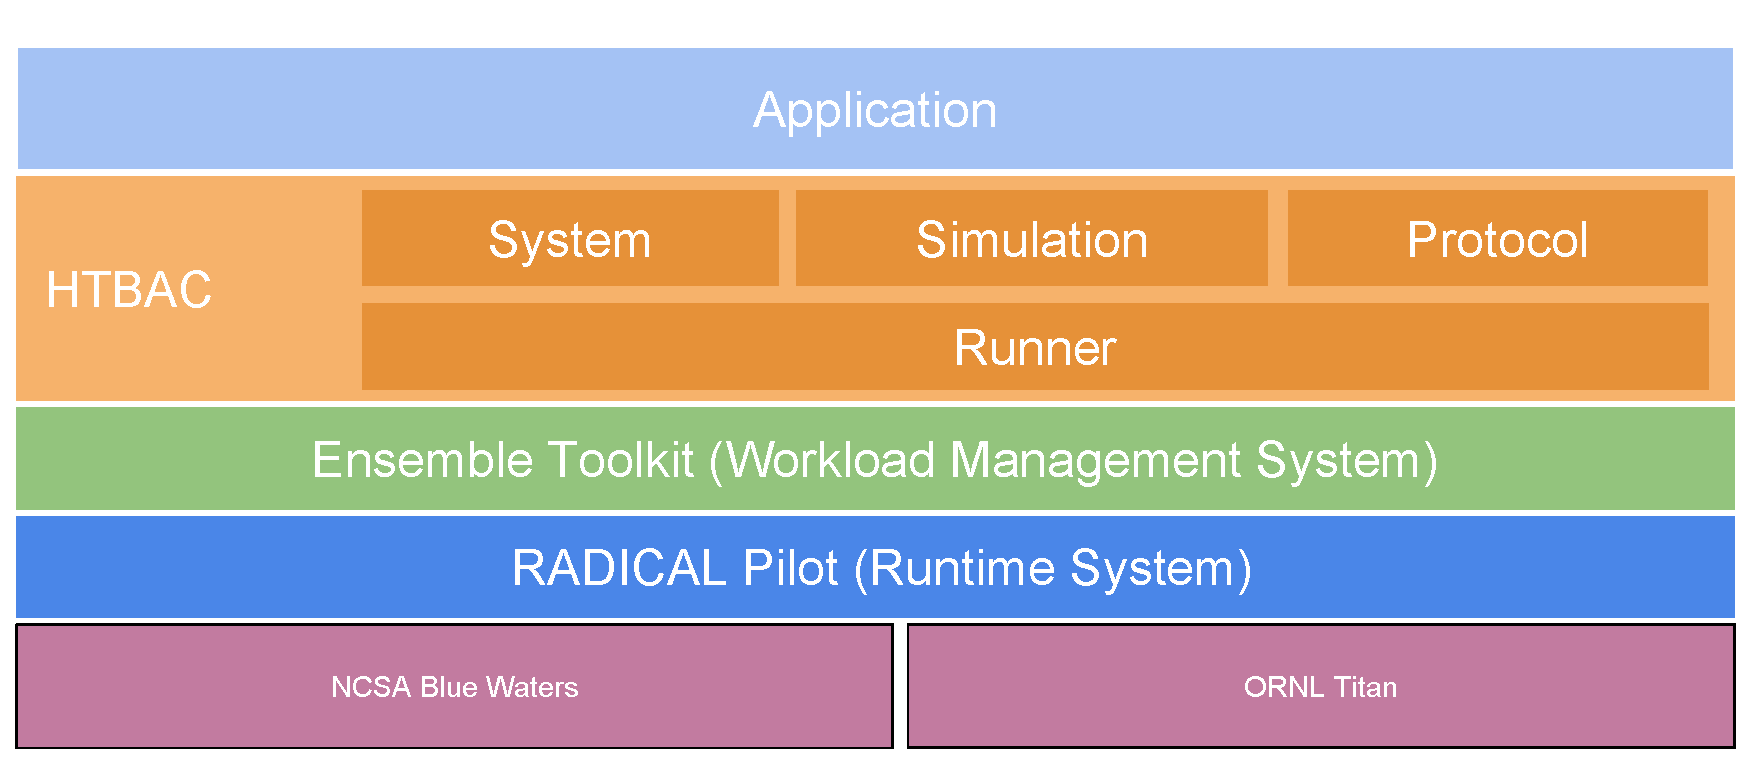
\includegraphics[width=\columnwidth]{figures/building_blocks.pdf}
%   \caption{Layered architecture of HTBAC, EnTK, and RP. The HTBAC API
%   exposes the Protocol component. Current protocols supporting the use cases
%   include ESMACS and TIES. EnTK serves as the workload execution system.
%   RADICAL-Pilot serves as the runtime system.}
% \label{fig:blockdiagram}
% \end{figure}




% ---------------------------------------------------------------------------
% \subsubsection{Workload Management and Runtime System}

% EnTK simplifies the process of creating ensemble-based applications with
% complex coordination and communication requirements. The EnTK API exposes the
% PST model which consists of three components\mtnote{I am not sure these are
% components. There is the risk to consider them architectural elements when
% they are not}: \textbf{Pipeline}, \textbf{Stage}, and \textbf{Task}. HTBAC
% promotes binding affinity \textbf{Protocols} as the user-facing construct,
% and uses the programming model defined by the Pipeline, Stage and Tasks model
% to express a specific protocol. \mtnote{The second part of this paragraph is
% inconsistent with the first: for example, see the use of PST and then
% `Pipeline, Stage and Task', or the use of protocols with capitalization
% (proper names are not plural) without differentiating them (it?) from those
% defined in EnTK via PST}

% Each HTBAC application aggregates one or more protocols. A workflow is
% comprised of $N_P$ instances of the P$^{th}$ protocol.

% each stage is a computational \textbf{task}, and the ordered aggregation of
% these stages alongside their dependencies as a
% \textbf{pipeline}~\cite{power-of-many17}.

% Sets of tasks with dependencies that determine the order of their execution
% are usually referred to as “workflows”.

% In section \ref{sec:science-drivers}, we described two examples of
% ensemble-based protocols for computing binding affinities.



% \begin{figure}
%   \centering
%   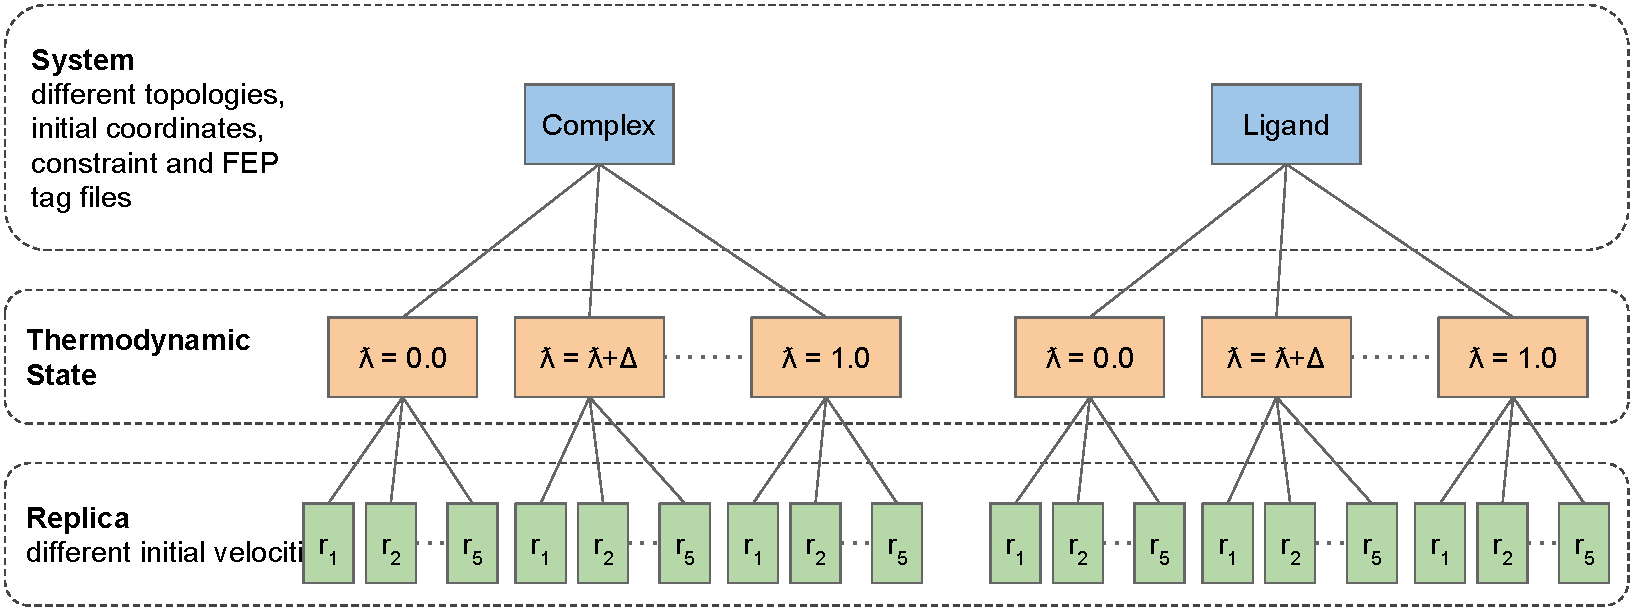
\includegraphics[width=\columnwidth]{figures/ties_workflow.pdf}
%   \caption{TIES workflow consisting a physical system, thermodynamic states
%   and replicas. Each replica is assigned a thermodynamic state. The workflow
%   is translated into an EnTK PST workflow. Construction Number of EnTK
%   Pipelines = 2 * (($\lambda$(max)/$\delta$) + 1) * 5 where $\lambda$(max) =
%   1 }
% \label{fig:ties_workflow}
% \end{figure}

  
\begin{figure}
  \centering
  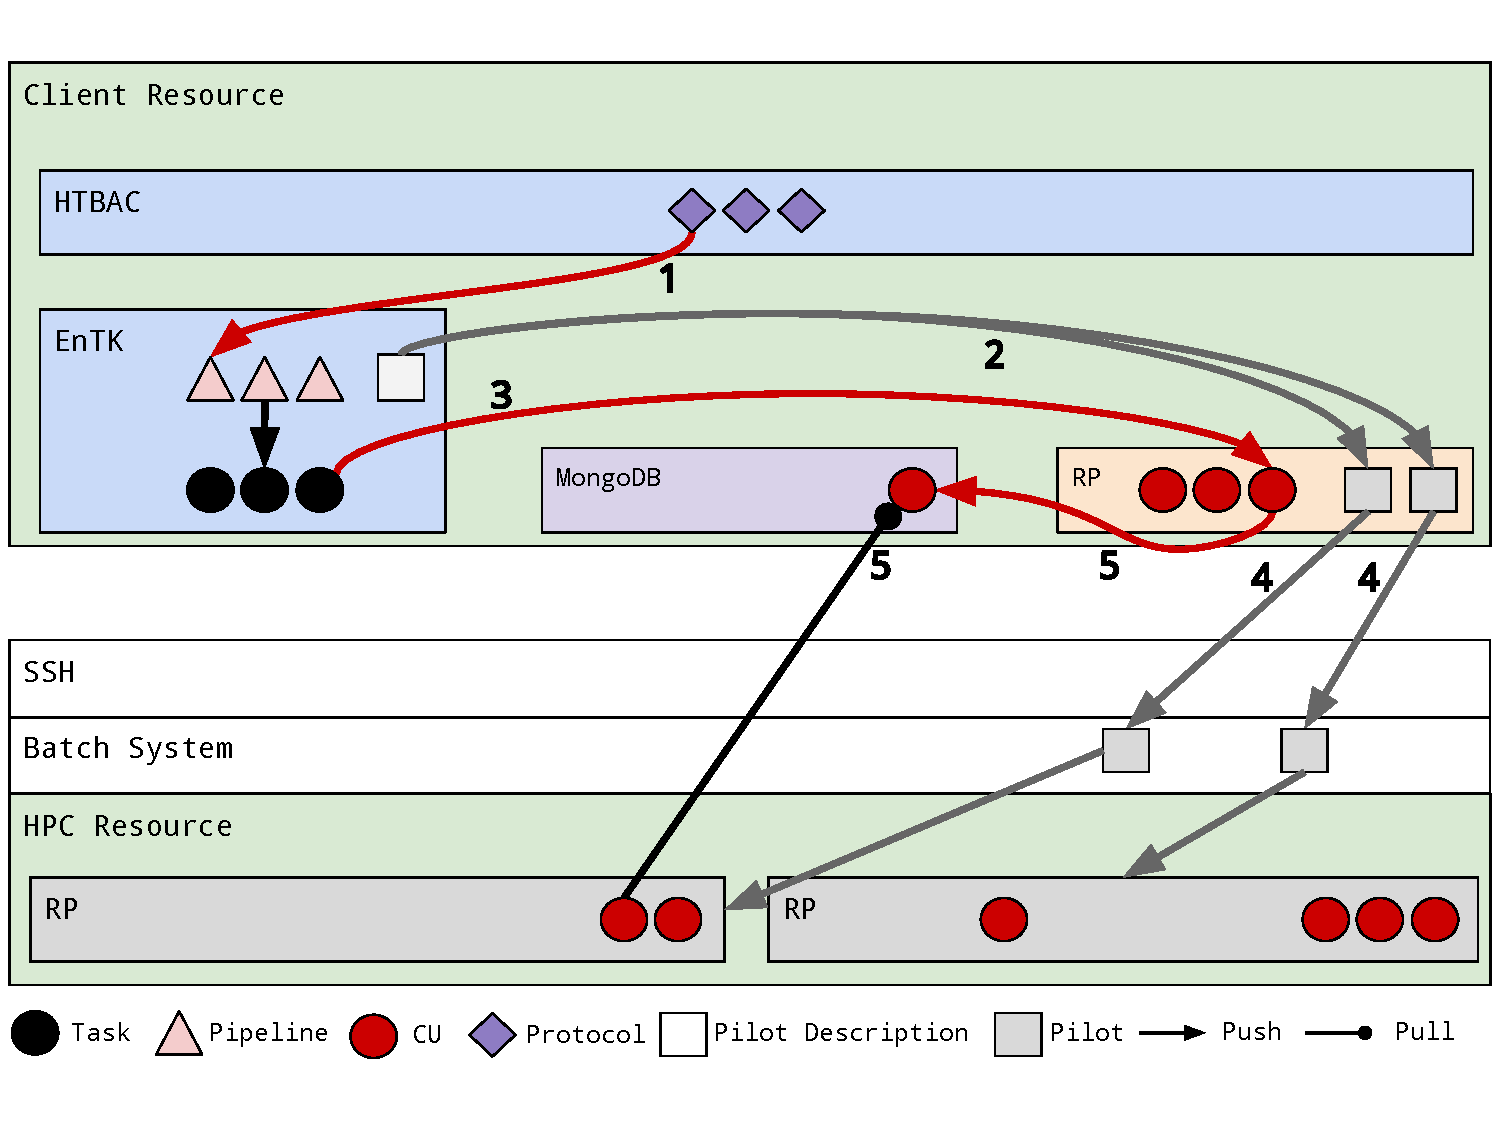
\includegraphics[width=\columnwidth]{figures/ht-bac-rp_integration.pdf}
  \caption{HTBAC, Ensemble Toolkit (EnTK) and RADICAL-Pilot (RP) integration 
  and execution sequence.\mtnote{Unreferenced figure.}\jdnote{does this figure
  help with execution model subsection?}}
\label{fig:integration}
\end{figure}

% Consistent with EnTK's programming model, HTBAC also uses the PST model to
% express {\bf Protocols}.

% Each protocol contains multiple stages with simulations and analysis tasks
% interspersed, in the most general case.

% programming model (that are consistent with the EnTK) to enable the user 

% HTBAC rests upon established middleware solutions~\cite{review_bb_2016},
% validated runtime abstractions~\cite{turilli2017comprehensive} for scalable
% execution, and customizes them for the computation of binding free
% energies.

% HTBAC derives many of the advantages of a lightweight, flexible domain
% specific workflow layer from its use of RADICAL-Cybertools (RCT) which are
% functionally well-defined and delineated middleware building blocks.
% RCT~\cite{review_bb_2016} are engineered to support extensible and scalable
% workflows across diverse computing platforms. The two primary RCT
% components that HTBAC depends upon are the Ensemble Toolkit (EnTK) and
% RADICAL-Pilot (RP).

% (so far, a workflow entails a maximum value of $P = 2$ and $N_P$=16, but in
% future work P will be greater $>$ 2).

% protocol, a user can scale protocol instances to study as many physical
% systems as desired.

% The specification of protocols and their parameters are passed by the user
% to the \textbf{Runner Handle} which translates the request to EnTK.

% In Section \ref{sec:related-work} we highlighted how an ensemble simulation
% approach can both aid sampling and improve uncertainty quantification for
% free energy calculations. Despite these crucial advantages, it remains
% non-trivial for field researchers to write biosimulation applications that
% involve individual protocols supporting multiple replicas, and by extension
% multiple protocols. With HTBAC, this burden is minimized by specifying the
% number of concurrent instances of the \textbf{Protocol} object. Moreover,
% the ability to generate multiple protocol instances enables the user to
% investigate a range of physical systems (i.e., drug candidates)
% concurrently.

% HTBAC allows the simple expression and concurrent execution of multiple
% distinct protocols, thereby enabling concurrent screening of drug
% candidates. HTBAC not only simplifies the expression of complex binding
% affinity protocols, but also provides hitherto unavailable capabilities,
% viz., the adaptive execution of these protocols, without any additional
% programming burden.

% Explain adaptive API and how it is passed to EnTK\mtnote{Please clearly
% identify comments in the text.}

% In turn, our adaptive execution implementation at the WMS focuses on
% supporting generality of adaptive workflows at the inter and intra-protocol
% level.

% \begin{figure}
%   \centering
%    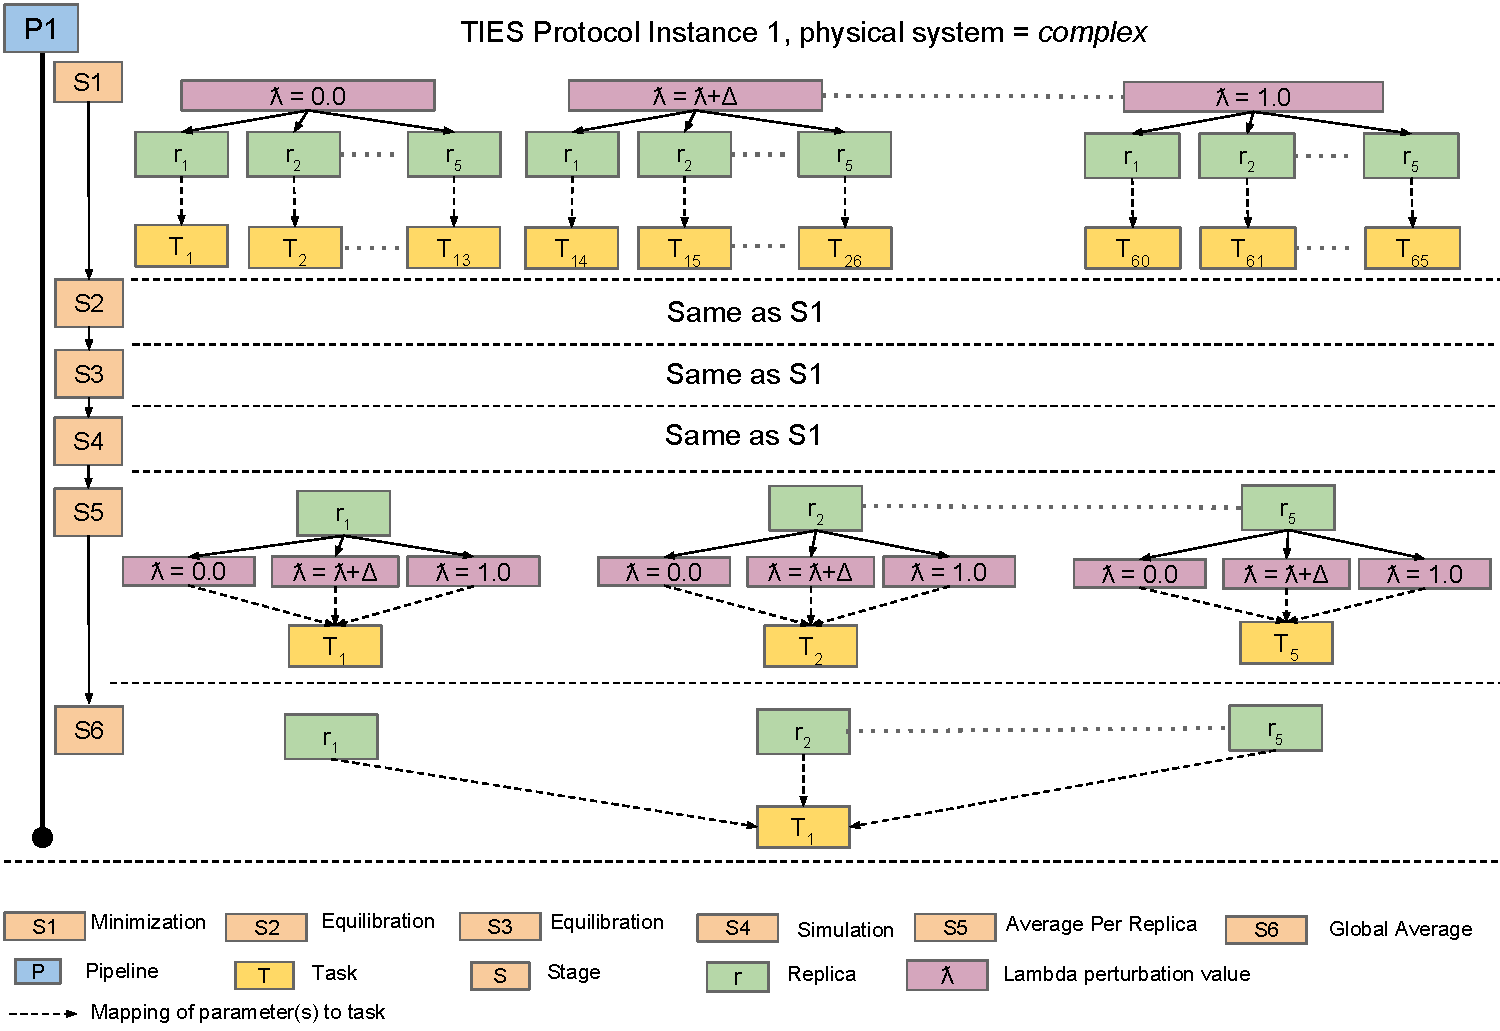
\includegraphics[width=\columnwidth]{figures/_TIES_EnTK_implementation.p
%    df}
%   \caption{TIES protocol expressed using the EnTK PST model. Each protocol
%   instance maps to a single Pipeline, comprised of Stage(s) which maintain
%   temporal order. Each Stage executes $n$ tasks, where $n$ represents the
%   number of unique lambda-replica combinations.}
% \label{fig:pst}
% \end{figure}


% \subsection{Scalability}

% Each protocol instance studies a single physical system i.e. drug
% candidate. By extension, the user is able to scale the number of concurrent
% protocol instances and therefore explore multiple concurrent drug
% candidates.

% ---------------------------------------------------------------------------


%\jhanote{Is this specific to the TIES protocol or to the protocol class.
%Needs clarification.} The same approach has been expanded to facilitate the
%creation of sub-ensembles where the simulation configuration is altered
%programatically. An example of this is the implementation ofthe TIES
%protocol, where the user controls the $\lambda$ parameter values used in
%simulatios to control which hybrid system states are sampled.

%A parameter, $\lambda \in [0, 1]$ is set for values between extremes and a
%simulation has to be run for every $\lambda$ value. The values form a
%function of energy and are integrated to obtain the desired results, the
%\emph{relative} binding free energy.

% ---------------------------------------------------------------------------
%\subsubsection{System}

%Systems This allows for multiple systems to be tested in the same
%\emph{single} run. A common scenario is the calculations of the binding
%affinity of a set of ligands with the same protein. System itself is just a
%collection of file paths pointing to descriptions of the system, like the
%system structure, topology etc. This class also provides the core/node
%requirments per single run, and reads some of the system descriptions from
%files to fill in the configuration settings.

%The Pipeline-Stage-Task (PST) framework developed by the Radical team
%(cite), and the Ensemble Toolkit (EnTK) built on top of it, offers a
%flexible way to express the molecular dynamics simulation workflows present
%in academia (cite) in terms of the radical pilot execution environment. Here
%we present a proposed mapping between the two (the PST and the MD layers)
%that is both simulation engine and protocol agnostic and allows for the
%compact expression of ensembles frequently used in binding affinity
%calculations.

%\subsection{Overview}

%The framework, called High Throughput Binding Affinity Calculator (HT-BAC),
%a python library, is made up of the following components: Workflow, Step,
%Ensembles and Simulation. These four object are all that is neccessary to
%describe the complex binding affinity caluculations in a generic way.

%\subsection{Workflow}

%The highest level abstraction is the Workflow. It is a container for the
%sequential units that are the simulation steps themselfs, and also contains
%meta-information about the job, like the resource description that the job
%will be running on, the total number of cores (nodes) required to fullfil
%the needs of the simulations and profiling mechanims to measure execution
%time.

% ---------------------------------------------------------------------------
%\jhanote{I don't these "description" should be subsections. Consider
%"\paragraph{}"}

%\subsection{Step}

%\jhanote{what is a step? It is unclear to the reader. Is "step"  construct
%within HTBAC or is this just a description of the pipeline?}

%The workflow containts an ordered list of \emph{steps}. Steps give
%\jhanote{order?} orderd to the basic building blocks of binding affinity
%calculations. Usually they are (i) minimization (some form of local
%optimization of atom coordinates), (ii) heating, (iii) equilibration and
%(iv) production run.

%Additionally there is one or more steps of analysis at the end. The key
%point, is that these steps \emph{have} to be run consecutively, as they are
%dependent on the previous one. This is ensured by the \texttt{Stage} objects
%of EnTK\@. Each step has list of \texttt{Ensemble}s and a
%\texttt{Simulation} object.

% ---------------------------------------------------------------------------

%$\subsection{Adaptability}

%Once we tackle the barrier between the local workflow creation and the
%remote execution, new features become availble, and readily usable by
%scientists. Intraprotocol adaptability is one such new feature.

% ---------------------------------------------------------------------------

% \subsubsection{Intraprotocol adaptability}

%while conceptually simple, tradiational execution patters used in academia
%makes this very hard. In HTBAC variables like replica size, specific lambda
%windows or simulatable system are settable on demand, the execution of which
%is automatically handeled by the library. To illustrate: a common scenario
%is the non adequate convergence of the statistical results after running a
%given number of replicas. In HTBAC the replica number can be changed, rerun
%and the results reevaluated. Additionally, logic can be written, to
%dynamically add more replicas until a given convergence tolerance has been
%reached.
